% -----------------------------------------------------------------------------
\documentclass[a4paper]{artikel3}
% -----------------------------------------------------------------------------
\paperheight = 29.70 cm  \paperwidth = 21.0 cm  \hoffset        = 0.46 cm
\headheight  =  0.81 cm  \textwidth  = 15.0 cm  \evensidemargin = 0.00 cm
\headsep     =  0.81 cm	 \textheight = 9.00 in  \oddsidemargin  = 0.00 cm					
% -----------------------------------------------------------------------------
\usepackage{enumerate}
\usepackage{amsfonts}
\usepackage{amsmath}
\usepackage{url}
\usepackage{graphicx}
\usepackage{float}
\usepackage[font=small,labelfont=bf]{caption}
\usepackage{setspace}
\usepackage{booktabs}
\usepackage[pdfpagemode=None,
		    colorlinks=true, 
		    urlcolor=blue, 
		    linkcolor=blue, 
		    citecolor=blue, 
		    pdfstartview=FitH]{hyperref}
% -----------------------------------------------------------------------------
\newtheorem{thm}{Theorem}
\newtheorem{cor}[thm]{Corollary}
\newtheorem{lem}{Lemma}
\newtheorem{prop}{Proposition}
\newtheorem{definition}[thm]{Definition}
\newtheorem{rem}[thm]{Remark}
\newtheorem{exm}[thm]{Example}
% -----------------------------------------------------------------------------
\newcommand{\norm}[1]{\left\Vert#1\right\Vert}
\newcommand{\abs}[1]{\left\vert#1\right\vert}
\newcommand{\set}[1]{\left\{#1\right\}}
\newcommand{\Real}{\mathbb R}
\newcommand{\eps}{\varepsilon}
\newcommand{\To}{\longrightarrow}
\newcommand{\mb}[1]{\mathbf{#1}}
\newcommand{\gb}[1]{\text{\boldmath$#1$}}
\newcommand{\ov}[1]{\overline{#1}}
\newcommand{\mml}{\{}
\newcommand{\mmr}{\}}
\newcommand{\lh}[1]{\widehat{#1}}
\newcommand{\pname}[1]{\textsc{#1}}
\newcommand{\lc}[1]{\mathscr{#1}}
\newcommand{\lcs}[1]{\ov{\mathscr{#1}}}
\newcommand{\lco}[1]{\overline{\mathscr{#1}}}
\newcommand{\lch}[1]{\widehat{\mathscr{#1}}}
\newcommand{\spi}{\ell}
\newcommand{\zf}[1]{z(#1)}
\newcommand{\R}{\mathbb{R}}

\usepackage{algorithm}
\usepackage[noend]{algpseudocode}

\algnewcommand{\Initialize}[1]{%
  \State \textbf{Initialize:}
  \Statex \hspace*{\algorithmicindent}\parbox[t]{.8\linewidth}{\raggedright #1}
}
% -----------------------------------------------------------------------------
\allowdisplaybreaks
\onehalfspacing
% -----------------------------------------------------------------------------

\graphicspath{ {Figures/} }

\begin{document}

% Title page
\begin{center}
{\Large \onehalfspacing \bf Solving Large-Scale Optimization Problems with ADMM}
\end{center}
\vspace{10pt}

% Use this if you work on your own and delete or comment over lines 72 - 77
%\begin{center}
%Hardworking Student\\
%{\textit{{\small{Aalto University School of Science, Department of Mathematics and Systems Analysis, 
%                 \{hardworking.student@aalto.fi\}}}}}
%\end{center}

% Use this if you work with a pair
\begin{center}
Christian Segercrantz, Tuukka Mattlar\\ 
{\textit{{\small{Aalto University School of Science, Department of Mathematics and Systems Analysis\\
%Aalto University School of Science, Department Computer Science\\
		         \{christian.segercrantz, tuukka.mattlar\}@aalto.fi}}}}
\end{center}

\section{Introduction} \label{sec:intro}
Large optimization problems are computationally heavy tasks. Moreover, having to consider multiple varying scenarios of a problem can easily increase the computational time required exponentially. Having efficient methods for solving large problems is therefore essential, as especially stochastic problems tend to quickly grow large in size. These kinds of problems do, however, usually display separability which may allow for algorithm modifications that allow the use of decompositions and parallelization.

This project aims to create an optimization algorithm making use of the alternating direction method of multipliers (ADMM). We will begin by discussing the motivation and theory behind the method and algorithm. Having discussed this, we continue with an in-depth walk-through of the algorithm and its application of it. We will then present our results, including results on time taken and iterations for different penalty term parameters used in the algorithm. Additionally, we compare the results to a classic deterministic method as well as convergence statistics. Finally, we discuss the results and conclusions that can be drawn from them and discuss potential future improvements.

The computations were performed on two separate platforms, these will be referred to as the cloud server and the local setup. The local setup runs Windows 10 build 19043.1319. The central processing unit (CPU) is an Intel Core i7-6700K, which has 4 cores with 2 threads each, overclocked to a clock speed of 4.00GHz. The PC has 16GB of rapid access memory (RAM) clocked at 2667 MHz. The cloud server used is the Aalto CS's JupyterLab server. The detailed information of this server is not available but the authors speculate that it runs a Unix-based operating system. The server is part of the Triton computing cluster. The Interior Point OPTimizer (Ipopt) was used as a solver in all cases.

\section{Background} \label{sec:background}
%Describe the ADMM and 
%ADNN's relevant technical details for the application at hand. 
%Provide a general pseudocode of ADMM and 
%provide a technical description of its steps based on the knowledge acquired in the course. 
%A discussion on stopping conditions and convergence would also be of value in this section.


\subsection{Augmented Lagrangian method of multiplies}
We start by considering the primal problem:
\begin{align}
    \text{min.} &f(x) \\
    \text{st.} &Ax = b
\end{align}
The general augmented Lagrangian for the problem can be formed as
\begin{align}
    L_{\mu} (x,v) = f(x) +\sum_{i=1}^l v_i h_i(x) + \mu \sum_{i=1}^l h_i(x)^2
    \label{fnc:ADMM}
\end{align}
where $(x,v)$ is the primal-dual pair.


The augmented Lagrangian method of multipliers (ALMM) combines the Lagrangian function and penalty terms with the perks of duality. Here, the penalty term allows for exact convergence with a finite penalty which is caused by the penalty term losing conditions of the dual function. The method of multipliers is basically a dual ascent method, but with the penalty parameter used to determine the step sizes. The alternating direction method of multipliers (ADMM), which is our main algorithm of interest, is a combinatorial variant of the ALMM.

\subsection{ADMM} \label{sec:ADMM}

ADMM is the alternating direction version of the ALMM as its primal and dual variables are updated in a sequential way. This separation of the primal and dual variables allows for the decomposition of the whole problem, in case the problem is separable. In fact, we can consider the following problem for the separated version:

\begin{align}
    \min_{x,y}.  & f(x)+g(y) \\
    \text{st.} &Ax +By = c
\end{align}

Compared to a standard linear problem, the problem is split into functions $f$ and $g$ and variables $x$ and $y$. This means that the problem is separable and allows for decomposition. Applying the ADMM method to optimization problems can provide an efficient solution since it makes use of the separation of the problem which further can allow for parallelization of the problem computation. Further assumptions of the problem will be discussed later. 

The problem can be further converted to a augmented Lagrangian form:
\begin{align*}
    \phi (x,y,v) = f(x)+g(z)+v^{\top} (c-Ax-By)+\mu (c -Ax - By)^2.
\end{align*}
This form of the problem can be solved using ADMM according to the pseudo-code \ref{euclid} where steps 3, 4, and 5 correspond to updating the variables. %For the primal variables, $x$ and $y$, we apply sequential minimization of the augmented Lagrangian function. For the dual variable $v$, we perform a gradient descent step to keep it optimal.

\begin{algorithm}[H]
    \caption{ADMM}\label{euclid}
    \begin{algorithmic}[1]
        \Initialize{Tolerance $\epsilon >0$, initial dual and primal solutions $v^0$ and $y^0$, $k=0$}
        \While{$|c-A \Bar{x}^k-B \Bar{y}^k|$ and $||y^{k+1}-y^{k}||> \epsilon$} 
        \State $\Bar{x}^{k+1} = \text{argmin } \phi_{\mu} (x, \Bar{y}^k, \Bar{v}^k)$
        \State $\Bar{y}^{k+1} = \text{argmin } \phi_{\mu} (\Bar{x}^k, y, \Bar{v}^k)$
        \State $\Bar{v}^{k+1} = \Bar{v}^k + \mu (c-A \Bar{x}^{k+1} - B \Bar{y}^{k+1})$
        \State $k = k +1$
        \EndWhile
        \Return{$(x^k,y^k)$}
    \end{algorithmic}
\end{algorithm}

In the algorithm \ref{euclid}, we first initialize the variables on row 1. Here, we introduce and set the tolerance parameter $\epsilon$ with a value greater than 0, declare the initial variables for the primal decision variables $x,y$, and finally set a counter for following the number of iterations.

In row 2 we start a while loop that waits for the convergence of the primal decision variables with the set tolerance. If the change between recurring iterations becomes small enough, the optima are achieved with the pursued precision.

On rows 3 and 4 we optimize both primal variables separately resulting in alternating direction, a key characteristic of the model. The value for $x^{k+1}$ purely just updates the state based on the previous iteration round so that the values of $y^{k+1}$ and $v^{k+1}$ can be achieved.

Finally, in row 5 we take into account the dual step by computing the dual optima based on the primal optima. Finally, in row 6, the iteration count is increased to keep track of the number of iterations.

\subsection{Convergence of ADMM}
In order for us to study the convergance of ADMM we need to discuss and state the following assumptions.% We make the following assumptions: 
\begin{enumerate}
    \item Functions $f$ and $g$ are convex, proper and closed. \cite{boyd2011distributed}
    \item For the augmented Lagrangian there exists a saddle point. \cite{boyd2011distributed}
\end{enumerate}
Based on the first assumption, we know that the augmented Lagrangian is solvable, i.e. there exists such $x$ and $y$ that minimize it. These values are not necessarily unique. The augmented Lagrangian will be finite for any saddle points $(x',y',v')$ which therefore implies that the saddle point $(x',y')$ is a solution \cite{boyd2011distributed}. Based on both assumptions, we know that a solution found from the augmented Lagrangian will fulfill the constraints of the original problem as the functions $f$ and $g$ will be finite. Additionally, strong duality holds for the problem, i.e., the primal and dual optimal solutions will be equal. Hence, the solution found for $y$ will be dual optimal. Due to these constraints, we will know that the (primal) residual, $r = Ax + By - c$, will converge towards 0 as k increases. In other words, the algorithm moves towards feasibility. Secondly, we can state that the original objective function value will also converge towards optimality. Lastly, the dual variable $v$ will converge towards its optimal value. 

\subsection{Optimality and stopping conditions of ADMM}
The necessary and sufficient optimality conditions for alternating  direction  method  of  multiplier problems are primal, $h(x) = 0 \implies Ax + By - c = 0$, and dual feasibility, $\nabla f(x) + A^\top v = 0$, $ \nabla g(y) + B^\top v = 0$ (in case the functions are differentiable). \cite{boyd2011distributed}. Since $y^k$ and $v^k$ always satisfy $ \nabla g(y^k) + B^\top v^k = 0$, we only need to look at the two other equations, i.e.
\begin{align}
    Ax + By - c &= 0 \label{eq:opt_cond1}\\
    \nabla f(x) + A^\top v &= 0. \label{eq:opt_cond2}
\end{align}
From equation \ref{eq:opt_cond1}, we can derive the residual $r^k = Ax^k + By^k - c$. From Equation \ref{eq:opt_cond2}, we can, by knowing that $x^{k+1}$ minimizes the augmented Lagrangian, transform it into 
\begin{equation}
    \nabla f(x^{k+1}) + A^\top v^{k+1} + \rho A^\top B (y^k-y^{k+1}) = 0
\end{equation}
where we will call $s^{k+1}=\rho A^\top B (y^k-y^{k+1})$ the dual residual. By making these two terms converge to zero, optimality can be archived. The proof that the ADMM algorithm will indeed make both the primal and dual residuals converge to zero is found in the references appendix \cite{boyd2011distributed}.

It has been seen that ADMM converges quickly close to the optimal solution, but slowly to a very high accuracy solution. Because of this, it's good to have reasonable stopping conditions. As stated earlier, the residuals are strongly tied to the convergence of the algorithm. Thus, basing the stopping criterion on the (scaled) residuals is reasonable. 
\section{Applications}

\subsection{The stochastic capacity expansion model}
We examine the following stochastic capacity expansion problem. 

\begin{align}
    &\text{min.}& & \sum_{i \in I} C_i x_i + \sum_{s \in S} P_s(\sum_{i \in I} \sum_{j \in J} F_{i,j} y_{i,j,s}+\sum_{j \in J} Q_j u_{j,s})& \label{eq:original_obj} \\
    &\text{st.}& & \sum_{i \in I} C_i x_i \leq B & \\
    &&& \sum_{j \in J} y_{i,j,s} \leq x_i, &\forall i \in I, \forall s \in S \\
    &&& \sum_{i \in I} y_{i,j,s} = D_{j,s}-u_{j,s}, &\forall j \in J, \forall s \in S \\
    &&& x_i \leq B_i, &\forall i \in I \\
    &&& x_i \geq o, &\forall i \in I \\
    &&&  y_{i,j,s} \geq 0, &\forall i \in I, \forall j \in J, \forall s \in S \\
    &&&  u_{j,s} \geq 0, &\forall j \in J, \forall s \in S \\
\end{align}
Here, $I$ is the set of suppliers, $J$ is the set of clients with unknown demand and $S$ represents the set of scenarios. Moreover, $D_{js}$ is the demand realization, $P_s$ associated scenario probabilities. $x_i$'s are reserving capacity amounts from supplier $j$ and $y_{ij,s}$'s the amount of capacity reserved from supplier $i$. Further, $u_{j,s}$ are not fulfilled demands in case capacity was not adequate and those come with a unit cost $Q_j$ and $f_{i,j}$'s are the unit costs to fulfill demand. Finally, a budget of $B_i$ capacity is available for all $i$ with a maximum overall budget of $B$.



\subsection{Applying ADMM to the stochastic capacity expansion model}
%Describe how ADMM can be specialized for the stochastic capacity expansion problem. 
To apply the problem in question to the ADMM algorithm we first identify the separability of the objective function. This allows the use of ADMM instead of ALMM.

In order for us to use the ADMM algorithm, we need to transform the problem into a augmented Lagragian form, as discussed earlier. % The augmented Lagragian function for the problem for each scenario $s$ is formed as
%\begin{equation}
%    L_s^{\rho} (x_s, y_s, z, v_s) = \sum_{i \in I}( (C_i+v_{i,s})x_i + \sum_{j \in J} (F_{i,j} y_{i,j} + Q_{j} u_j + \frac{\rho}{2}(x_i-z_i)^2 ) )
%\end{equation}
In the below equation, we can see the different steps of the pseudo-code from earlier. Equation \ref{eq:admm_obj} is the objective function that is to be minimized. Instead of the tolerance in the while part, line 2, in the pseudo-code, will we use a modified version seen in Equation \ref{eq:admm_tol}. This tolerance consists of a scenario probability-weighted sum of the penalty term times the norm of $x_s$ and z.

\begin{alignat}{3}
	&\text{Based on}& &\phi (v)= \text{min} \sum_{s \in S} P_s L_s^{\rho} (x_s, y_s, z, v_s)\label{eq:admm_phi} \\
	&\text{min. } & L_s^{\rho} (x_s, y_s, z, v_s) &= \sum_{i \in I}( (C_i+v_{i,s})x_i + \sum_{j \in J} (F_{i,j} y_{i,j} + Q_{j} u_j + \frac{\rho}{2}(x_i-z_i)^2 ) ) \label{eq:admm_obj} \\
	&&&=\sum_{i \in I} (C_i+v_{i,s})x_i +\sum_{i \in I} \sum_{j \in J} F_{i,j} y_{i,j}   \sum_{j \in J}  Q_{j} u_j+ \sum_{i \in I} \frac{\rho}{2}(x_i-z_i)^2 \\
	&\text{x-step } &  x^{k+1} &= \text{argmin } L_{\rho} (x, y^k) \label{eq:admm_xstep} \\
	&\text{z-step } & z^{k+1} &= \sum_{s \in S} p_s x_s^{k+1}  \label{eq:admm_zstep}\\
	&\text{v-step } & v_s^{k+1} &= \sum_{s \in S} v_S^k + \rho (x_S^{+1} - z^{k+1})  \label{eq:admm_vstep} \\
	&\text{Tolerance } & \epsilon &> \sum_{s \in S} p_s \rho || x_s^{k+1} - z^k||_2  \label{eq:admm_tol}
\end{alignat}

In more detail, in Equation \ref{eq:admm_phi} we introduce the augmented Lagrangian based on the objective function, seen in Equation \ref{eq:original_obj}, with a penalty term, as was seen in Algorithm \ref{euclid}.


The x-step in Equation \ref{eq:admm_xstep} is purely updated based on the last iteration of new $z,v$ values. This step, therefore, updates the $x$ in order to compute the other steps.

Since the $z$-variable is responsible for the nonanticipativity of the variable x, we simply update it by taking the weighted sum of the newly obtained x-values. This can be seen in Equation \ref{eq:admm_zstep}.

Finally, the v-step is represented in Equation \ref{eq:admm_vstep} representing the dual solution by utilizing the gradient descent method with a penalty step size $\rho$.

The tolerance condition for ending, in the Equation \ref{eq:admm_tol} is obtained from the sum of the squares of the residuals $|| x_s^{k+1} - z^{k+1}||_2^2 + ||z^{k+1}-z^k||^2_2 = ||x_s^{k+1}-z^k||_2^2$, which is then squared. Moreover, the value is multiplied with the penalty step size $\rho$ and the scenario probability $p_s$ is taken into account.


%Provide a detailed description of each of the ADMM steps, relating to the pseudocode presented in the previous section. Provide all details necessary for implementing this variant of ADMM for the problem you are solving.

\section{Discussion and conclusions}
%Describe the results obtained in terms of number of iterations. Assess the ADMM implementation with respect to values used for the penalty term ρ and solution obtained when compared to that you obtain by solving the full-scale model (i.e., the model without decomposition). Present a structured performance comparison with respect to the total computational time and the number of iterations before converging to a solution for different values of the penalty term ρ within the interval [0.5, 100] 

%Simple examples show that ADMM can be very slow to converge to high accuracy. However, it is often the case that ADMM converges to modest accuracy—sufficient for many applications—within a few tens of iterations. This behavior makes ADMM similar to algorithms like the conjugate gradient method, for example, in that a few tens of iterations will often produce acceptable results of practical use. However, the slow convergence of ADMM also distinguishes it from algorithms such as Newton’s method (or, for constrained problems, interior-point methods), where high accuracy can be attained in a reasonable amount of time. While in some cases it is possible to combine ADMM with a method for producing a high accuracy solution from a low accuracy solution [64], in the general case ADMM will be practically useful mostly in cases when modest accuracy is sufficient. Fortunately, this is usually the case for the kinds of large-scale problems we consider. Also, in the case of statistical and machine learning problems, solving a parameter estimation problem to very high accuracy often yields little to no improvement in actual prediction performance, the real metric of interest in applications.

% Conclusions:
% - Better on large instances (to be expected)
% - Dependent on setup
% - Probably very efficient when actually parallel computations used

The ADMM algorithm was run using a max iteration limit of $N=200$, a tolerance of $\epsilon=10^{-1}$, and a varying $\rho$. For each iteration, the time taken in seconds and the iteration amount needed was recorded. The algorithm was run on small, medium, and large instances. The instance specifications can be seen in Table \ref{tab:instance_specs}. The algorithm was run for each instance using $rho \in [0.5,99.5]$ with a step size of 1. The number of iterations as a function of $\rho$ can be seen in Figure \ref{fig:iterations_cloud}. The results of the time, with the deterministic model as a reference, can respectively be seen in Figure \ref{fig:times_cloud}. During all of the runs, the algorithm converged in less than $N$ iterations, in fact, all runs were completed in less than 7 iterations. All runs for Figures \ref{fig:iterations_cloud} and \ref{fig:times_cloud} were done on the cloud setup discussed in Section \ref{sec:intro}.

\begin{table}[h]
    \centering
    \caption{The specifications used to generate the instances.}
    \label{tab:instance_specs}
        \begin{tabular}{l|l|l|l|}
        \cline{2-4}
                                              & \textbf{Suppliers} & \textbf{Clients} & \textbf{Scenarios} \\ \hline
        \multicolumn{1}{|l|}{\textbf{Small}}  & 15                 & 20               & 50                 \\ \hline
        \multicolumn{1}{|l|}{\textbf{Medium}} & 15                 & 20               & 75                 \\ \hline
        \multicolumn{1}{|l|}{\textbf{Large}}  & 15                 & 20               & 100                \\ \hline
    \end{tabular}
\end{table}

\begin{figure}[H]
\centering
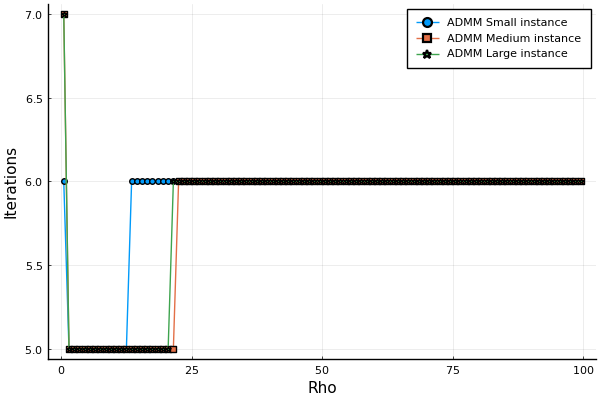
\includegraphics[width=0.80\textwidth]{iterations_cloud.png}
\caption{The number of iterations $k$ as a function of $\rho$. The ADMM ran for values between 0.5 and 95.5 with a step size of 1. The deterministic models as a reference. The simulations were run on the cloud setup.}
\label{fig:iterations_cloud}
\end{figure}

\begin{figure}[H]
\centering
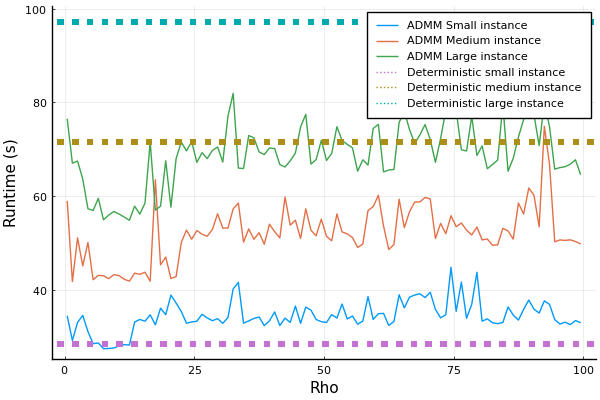
\includegraphics[width=0.80\textwidth]{times_cloud.png}
\caption{The run time until convergence  as a function of $\rho$. The ADMM ran for values between 0.5 and 95.5 with a step size of 1. The deterministic models as a reference. The simulations were run on the cloud setup.}
\label{fig:times_cloud}
\end{figure}


We begin by examining the number of iterations, visualized in Figure \ref{fig:iterations_cloud}. Overall the runs, the algorithm only resulted in three distinct iteration amount values, 5, 6, or 7. For the very lowest values of $\rho$, the solving took 7 iterations. For values in the range [1.5, 20.5], the medium and large instances needed 5 iterations. The small instance converged with 5 iterations in the interval [1.5,12.5]. For all other runs, the algorithm needed 6 iterations to converge. We can, therefore, say that there is no clear effect of the penalty term $\rho$ on the iteration amount needed for convergence. 

Figure \ref{fig:times_cloud} displays a similar story. We can see that the time needed for the algorithm to converge does not seem to have much dependence on the size of rho. There seem to be a few numbers that perform more poorly for the algorithm, but this can be contributed to software and hardware-related technical specifications especially since each step was only computed once. The figure additionally displays the deterministic full model. We can see that the ADMM runs mostly fall between the time needed for the deterministic model to solve the small and medium instances. This is a somewhat expected result since the ADMM excels at solving larger problems. We can see that on average the large instance is solved 1.3 times faster when using the ADMM algorithm than when using the deterministic model. However, the small instance is solved, in all but for a few $\rho$ values, faster using the deterministic model.

One of the strengths of ADMM lies in the decomposition of the problem, into separate parts that can be computed separately. In other words, the problem is parallelizable. However, the technical implementation of the algorithm in this project does not make us of that at all. In our code, we iterate through all of the scenarios three separate times for each (except for the last run, which only uses two runs) scenario $s$. In particular, one of the loops is constantly solving the optimization sub-problem, which is the heaviest part of the code. There is naturally some overhead that is not affected by the parallelization, but for the most part, the code would be sped up by as many threads that could be used for the computation.

An aspect that was not investigated in this work is the effect of the size of the tolerance $\epsilon$. Since the ADMM algorithm quickly converges close to the optimal solution but slowly to a high accuracy solution \cite{boyd2011distributed}, defining $\epsilon$ well could save a lot of time. In real-life scenarios, a close to accurate number is often enough, especially if it speeds up the process by a large portion.

\begin{figure}[H]
\centering
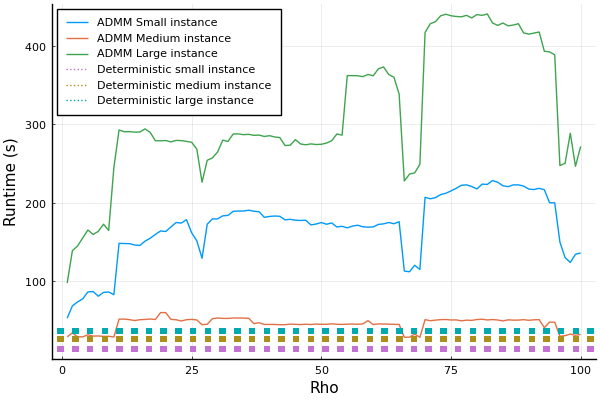
\includegraphics[width=0.80\textwidth]{times_local.png}
\caption{Same conditions as \ref{fig:times_cloud}, but the simulations were run on the local setup.}
\label{fig:times_local}
\end{figure}

Figure \ref{fig:times_local} shows the same algorithm with the same specifications ran on the local setup discussed in Section \ref{sec:intro}. We can see that the results vary widely from that of the cloud setup: the run time on ADMM clearly seems to slow down as the function of $\rho$ and all the ADMM solutions are around a magnitude slower than their deterministic ones. Additionally, the local setup solves the deterministic models way faster than the cloud setup. This indicates that knowledge of hardware, software, and solver specifications are important to know in order to determine if the choice of algorithm is good. For the local setup case, it does not seem to be worth building an extensive ADMM model that is slower than the full deterministic model in the studied case.

\bibliography{bibtex}{}
\bibliographystyle{plain}

\end{document} 